% !TEX root=../thesis.tex

\chapter{Background}
\label{chapter:background}


%Piloting map service for navigating in punctuality analysis for trains

A train network is a complex system. Almost every running train have the 
possibility to affect almost every other train running in the system.  When you look at a busy area, such as a major city and it's closest
area, a great deal of material can be on the move at any given time on a
rail network with limited capacity. This leads to limited time slots for each 
train and every problem can lead to major delays.

Even though one train may be experiencing delay, this delay may be part of a
sequence of problems that can be tracked back to a seemingly unrelated part of
the the network and a perhaps a bad decision there\cite{cule2011mining}. \\

As Landex\cite{landex2009gis} says, there exist few GIS-approaches concerning
visualization of railroad capacity. Both the visualizations shown by Landex and
in Section \vref{section:backgroundExamples} only seems to take into consideration if
the trains are delayed, and the amount of delay. 

However, to minimize the delays all over the rail network, it may be necessary
to not only see that certain routes are delayed but also why it is delayed. To
be able to understand this, you need to be able to mine data from the rail
network administrator and a good visualization tool to present it. 

\pagebreak
\section{Examples}
\label{section:backgroundExamples}

\subsection{Zugmonitor}
\label{subsection:zugmonitor}

In the Zugmonitor (see \vref{fig:zugmonitor}) example each long-distance 
trains in the German railway network has been plotted as a arrow on a German 
map. To illustrate the punctuality of each train, a colored circle has been 
added to each arrow if the train is delayed with varying color depending on 
how big the delay is. It has also been implemented a time line functionality 
to see how the trains are on each step of the routes. This time line 
functionality has both a play forward function and manually drag along the 
time line.

\begin{figure}[!htbp]
	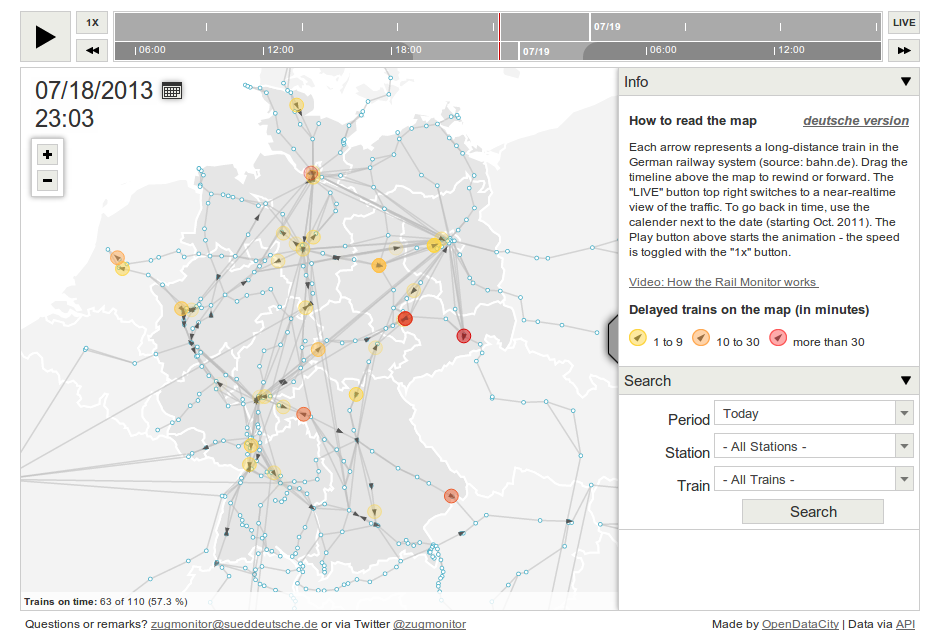
\includegraphics[width=\textwidth,center]{zugmonitor.png}
	\caption[Zugmonitor]{Zugmonitor \cite{zugmonitor}}
	\label{fig:zugmonitor}
\end{figure}
\pagebreak

\subsection{Vaguely live map of trains in the United Kingdom}
\label{subsection:ukLiveMap}

This is a map which plots the relative location of each train in the United
Kingdom (see \vref{fig:ukLiveMap}). The plot fetches the departure time from the 
National Rail website and calculates the relative location. The plot does not
indicate whether or not the trains are on schedule or delayed, this must be
done either manually or for instance checking a time table\cite{trainTimesUK}.
Both the map and time table is developed on hobby basis by the same person. 

\begin{figure}[!htbp]
	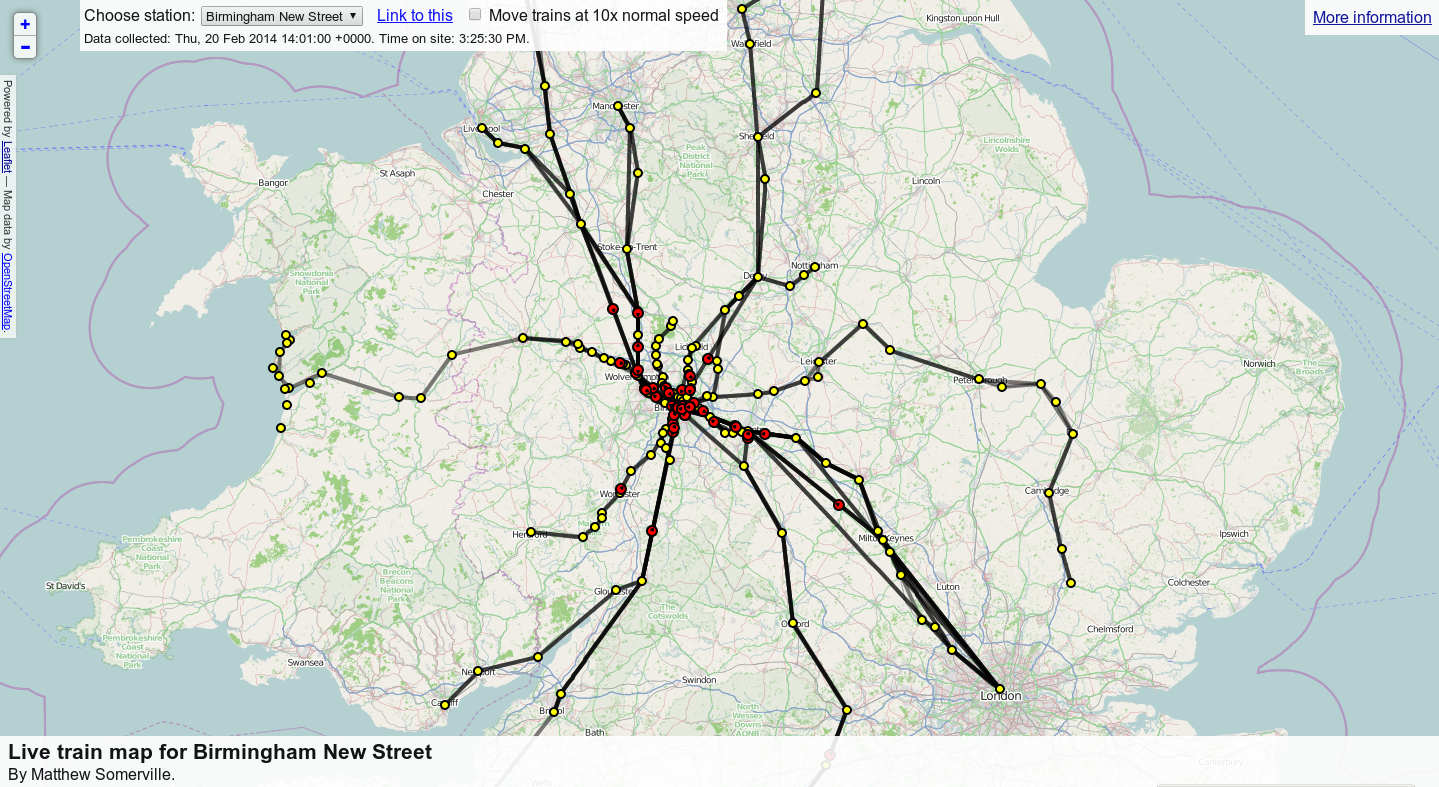
\includegraphics[width=\textwidth,center]{live-train-map-for-Birminingham-new-street.png}
	\caption[Vaguely live map of trains in the United Kingdom]{Vaguely live map of trains in the United Kingdom \cite{ukLiveMap}}
	\label{fig:ukLiveMap}
\end{figure}
\pagebreak

\subsection{MUNI Light Rail}
\label{subsection:muniLightRail}

This a train graph based on the N-Judah line on the Muni Metro light rail line in San Francisco (see \vref{fig:muniLightRail}). 
This chart plots the schedule of the each train and the actual time each train 
uses. The chart auto updates each 10 seconds, and combined with being able 
to spot the difference between the schedule and the actual time, makes it easy 
spot the delay of each train. As with \vref{subsection:ukLiveMap} it has been 
developed on a hobby basis.

\begin{figure}[!htbp]
	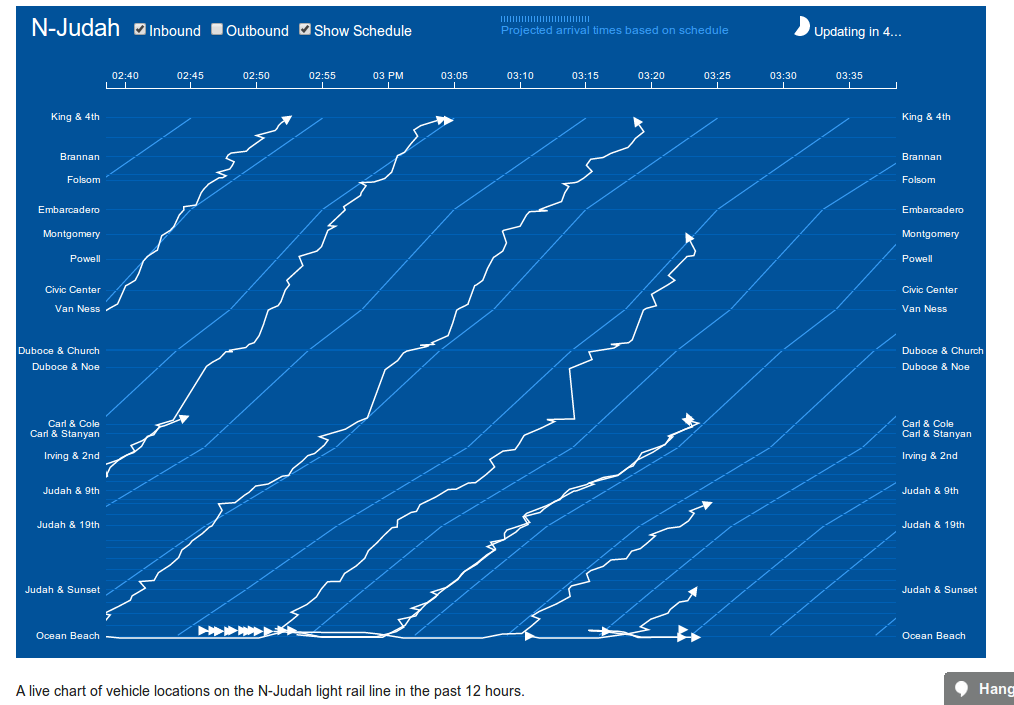
\includegraphics[width=\textwidth,center]{visualizing-transit-delays.png}
	\caption[Visualizing transit delays]{Visualizing transit delays \cite{muniLightRail}}
	\label{fig:muniLightRail}
\end{figure}
\pagebreak


\subsection{MiseryMap}
\label{subsection:zugmonitor}

The MiseryMap (see \vref{fig:miserymap}) shows how much different airports and 
the routes between them are delayed. It also have a playback function to see
how the delays are throughout the day. This plot also shows some weather so it
may be possible to spot if the delays to be blamed on uncontrollable
conditions. 

\begin{figure}[!htbp]
	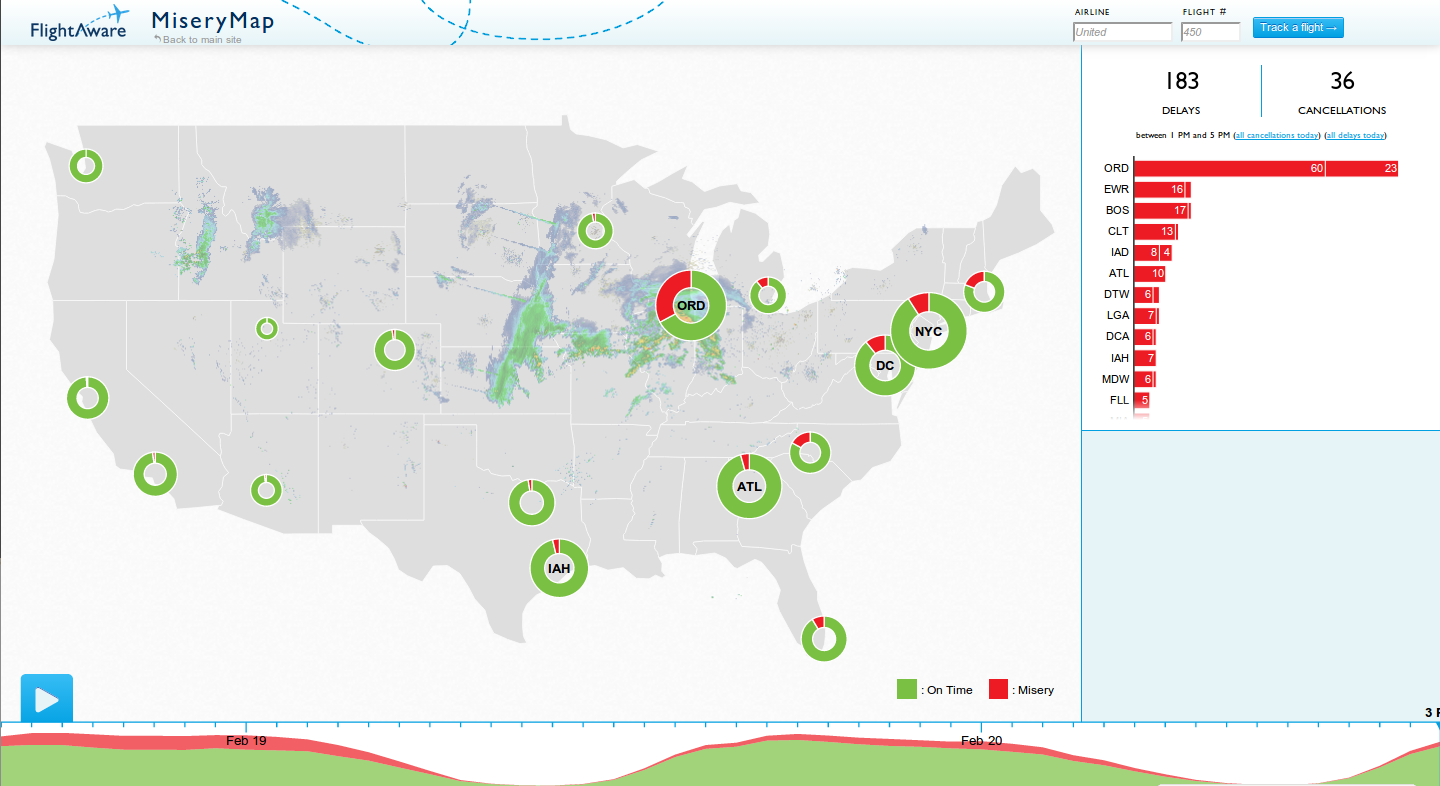
\includegraphics[width=\textwidth,center]{MiseryMap.png}
	\caption[MiseryMap]{MiseryMap \cite{flightAware:MiseryMap}}
	\label{fig:miserymap}
\end{figure}
\pagebreak
 
